\section{Geometry}



\subsection*{Vector3d}

\begin{frame}[fragile]
  \frametitle{Specimen Directions - The \MTEX Class \texttt{\bf vector3d}}

  Definition:

\begin{lstlisting}
v = vector3d(x,y,z)             % Cart. coordinates
v = vector3d('polar',theta,rho) % polar coordinates
v = xvector                     % predefined vector
\end{lstlisting}

  \medskip

  \begin{columns}
    \begin{column}{8.5cm}

      Calculations:

\begin{lstlisting}
v = [xvector,yvector]; w = v(1);
v = 2*xvector - yvector;
\end{lstlisting}

    \medskip

    Basic Functions:

\begin{lstlisting}
angle(v1,v2), norm(v)
dot(v1,v2), cross(v1,v2)
[theta,rho] = polar(v)
\end{lstlisting}
  \end{column}
  \begin{column}{3cm}
   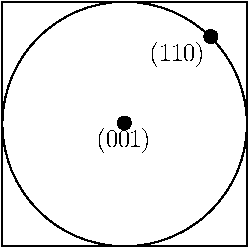
\includegraphics[width=3cm]{pic/vector3d}
  \end{column}
\end{columns}



\end{frame}

\subsection*{quaternion}


\begin{frame}[fragile]
  \frametitle{Rotations - The \MTEX Class \texttt{\bf rotation}}

Definition:

\begin{lstlisting}[mathescape=true]
rot = rotation('Euler',$\phi_1$,$\Phi$,$\phi_2$,'Bunge')
rot = rotation('axis',v,'angle',$\omega$)
rot = rotation('matrix',R)
rot = rotation('fibre',$u_1$,$v_1$,'resolution',5*degree)
rot = rotation('map',$u_1$,$v_1$,$u_2$,$v_2$) % $\mathbf{gu}_1=\mathbf{v}_1,\mathbf{gu}_2=\mathbf{v}_2$
rot = rotation('quaternion',a,b,c,d)
\end{lstlisting}

Euler angle conventions: Bunge, Matthies, Roe, Kocks, Canova


\begin{columns}
  \begin{column}{8.5cm}

    Calculations:

\begin{lstlisting}
v = rot * u    % apply rot to u
u = rot \ v    % inverse(rot)*v
rot = rot1 * rot2
\end{lstlisting}

    Basic Functions:

\begin{lstlisting}[mathescape=true]
angle(rot), axis(rot)
angle(rot1,rot2), inverse(rot)
[$\phi_1$,$\Phi$,$\phi_2$] = Euler(rot,'Bunge')
\end{lstlisting}


  \end{column}

  \begin{column}{3cm}
    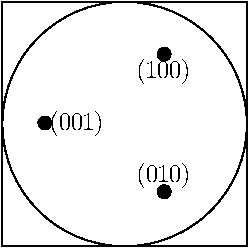
\includegraphics[width=3cm]{pic/quaternion}
  \end{column}

\end{columns}
\end{frame}



\subsection*{Symmetry}
\begin{frame}[fragile]
  \frametitle{Crystal Symmetries - The \MTEX Class \texttt{\bf symmetry}}

  Definition:

\begin{lstlisting}
S = symmetry('triclinic',[a,b,c],[alpha,beta,gamma])
S = symmetry('-3m',[a,b,c],/+'a||x'+/);
S = symmetry('O');
\end{lstlisting}

\medskip

\begin{columns}
  \begin{column}{8.5cm}

Load Symmetry from CIF file:

\begin{lstlisting}
symmetry('quartz.cif')
\end{lstlisting}

\medskip

    Basic Functions:

\begin{lstlisting}
symmetrise(v,S)
symmetrise(rot,CS,SS)
rotation(S)
project2FundamentalRegion(v,CS)
project2FundamentalRegion(rot,CS,SS)
\end{lstlisting}
  \end{column}

  \begin{column}{3cm}
    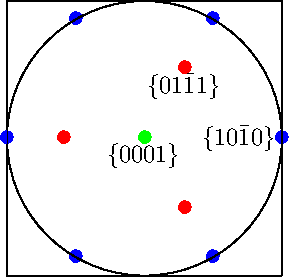
\includegraphics[width=3cm]{pic/sym}
  \end{column}

\end{columns}

\end{frame}

\subsection*{Miller}

\begin{frame}[fragile]
  \frametitle{Crystal Directions - The \MTEX Class \texttt{\bf Miller}}

  Definition:

\begin{lstlisting}
h = Miller(v,CS);
h = Miller(1,0,0,CS);
h = [Miller(1,1,-2,3,CS),Miller(0,1,-1,0,CS)]
\end{lstlisting}

\medskip

\begin{columns}
  \begin{column}{8.5cm}

    Calculations:

\begin{lstlisting}
h1 + h2
rot * h     % apply rot on h
\end{lstlisting}

    Basic Functions:

    \begin{onlyenv}<1>
\begin{lstlisting}
eq(h1,h2), angle(h1,h2)
symmetrise(h)  % get all equivalent
plot([h1,h2],'all')
\end{lstlisting}
    \end{onlyenv}

	\end{column}

  \begin{column}{3cm}
    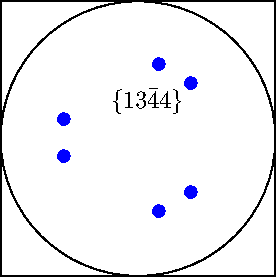
\includegraphics[width=3cm]{pic/miller}
  \end{column}
\end{columns}


	\begin{onlyenv}<2>

		\lstset{stringstyle=\color{red},emph={antipodal},emphstyle=\em\color{red}}

	\begin{lstlisting}
	eq(h1,h2,`antipodal`), angle(h1,h2,`antipodal`)
	symmetrise(h,`antipodal`)
	plot([h1,h2],'all',`antipodal`)
	\end{lstlisting}


    \end{onlyenv}


\end{frame}



\begin{frame}[fragile]
  \frametitle{Orientations - The \MTEX Class \texttt{\bf orientation}}

Definition:

\begin{lstlisting}[mathescape=true]
ori = orientation(rot,CS,SS)
ori = orientation('Euler',$\phi_1$,$\Phi$,$\phi_2$,CS,SS,'Bunge')
ori = orientation('Miller',[h k l],[u v w],CS,SS)
ori = orientation('brass',CS,SS)
\end{lstlisting}

\begin{columns}
  \begin{column}{8.5cm}

    Calculations:

\begin{lstlisting}
r = ori * h, h = ori \ r
ori = rot * ori
\end{lstlisting}

    Basic Functions:

\begin{lstlisting}[mathescape=true]
angle(ori),angle(ori1,ori2),axis(ori)
symmetrise(ori),eq(ori1,ori2)
project2FundamentalRegion(ori,ref_ori)
[$\phi_1$,$\Phi$,$\phi_2$] = Euler(or,'Bunge')
\end{lstlisting}

  \end{column}

  \begin{column}{3cm}
    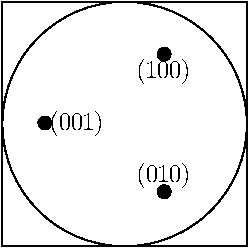
\includegraphics[width=3cm]{pic/quaternion}
  \end{column}

\end{columns}
\end{frame}



\subsection*{Exercises}

\begin{frame}

  \begin{Exercise}
    Consider trigonal crystal symmetry.

  \begin{enumerate}[a)]
    \item Find all crystallographic directions symmetrically equivalent to $h
      = (1, 0, \bar 1, 0)$ (Miller indices)!
    \item Find crystallographic directions such that the number of their
      crystallographic equivalent directions on the upper hemisphere (without
      equator) is 1, 3, and 6, when including antipodal symmetry!
    \item Consider the orientation given by the Euler angles $(30\degree,
      90\degree, 90\degree)$ in Bunge convention. Give the Euler angles of
      all symmetrically equivalent orientations!
    \item Which positions in the (0,0,0,1) - pole figure corresponds to the
      above orientation. Which crystal direction is rotated by this
      orientation to the specimen direction (0,0,1)?
    \item Construct an orientation that rotates the crystallographic
      directions $(0,0,0,1)$ and $(2,\bar 1,\bar 1,0)$ onto the specimen
      directions $(1,0,0)$ and $(0,1,0)$, respectively. Describe the rotation
      by axis and angle.
    \end{enumerate}

  \end{Exercise}

\end{frame}

%%% Local Variables:
%%% mode: latex
%%% TeX-master: "main"
%%% End:
